\documentclass[11pt]{report}

\usepackage[landscape]{geometry}
\usepackage{tikz}
\pagenumbering{gobble}

\begin{document}

\center
\scalebox{3}{
\begin{tikzpicture}[block/.style={rectangle,text width=6em,text centered,minimum height=9mm}]
\def\hZero{1}
\def\hOne{1.5}
\def\hTwo{2}
\def\hThree{2.5}
  \draw[->] (-1,0) -- (4,0) node[right] {$x$};
  \draw[->] (0,-0.5) -- (0,4) node[above] {$y$};
  %\draw[help lines] (-6,-5) grid (8,6);
\draw[scale=1,domain=-1:4,smooth,variable=\x,blue] plot ({\x},{1/2*\x+1});
\draw (0,\hZero) circle (0.1cm);
\path
(-0.5,\hZero) node [block] (spy1) {$sk_1$}
;
  %\draw[scale=0.5,domain=-3:3,smooth,variable=\y,red]  plot ({\y*\y},{\y});
\end{tikzpicture}
}

\newpage

\scalebox{3}{
\begin{tikzpicture}[block/.style={rectangle,text width=6em,text centered,minimum height=9mm}]
\def\hZero{1}
\def\hOne{1.5}
\def\hTwo{2}
\def\hThree{2.5}
  \draw[->] (-1,0) -- (4,0) node[right] {$x$};
  \draw[->] (0,-0.5) -- (0,4) node[above] {$y$};
  %\draw[help lines] (-6,-5) grid (8,6);
\draw[scale=1,domain=-1:4,smooth,variable=\x,blue] plot ({\x},{1/2*\x+1});
\draw (0,\hZero) circle (0.1cm);
\draw (1,\hOne) circle (0.1cm);
\draw (2,\hTwo) circle (0.1cm);
\draw (3,\hThree) circle (0.1cm);
\path
(-0.5,\hZero) node [block] (spy1) {$sk_1$}
(-0.5,\hOne) node [block] (spy1) {$\sigma_{1,1}$}
(-0.5,\hTwo) node [block] (spy1) {$\sigma_{2,1}$}
(-0.5,\hThree) node [block] (spy1) {$\sigma_{3,1}$}
(1,-0.5) node [block] (spy1) {1}
(2,-0.5) node [block] (spy1) {2}
(3,-0.5) node [block] (spy1) {3}
;

\begin{scope}[every path/.style=draw,densely dotted,thick]
\path (1,\hOne) -- (0,\hOne);
\path (1,\hOne) -- (1,0);
\path (2,\hTwo) -- (0,\hTwo);
\path (2,\hTwo) -- (2,0);
\path (3,\hThree) -- (0,\hThree);
\path (3,\hThree) -- (3,0);
\end{scope}
  %\draw[scale=0.5,domain=-3:3,smooth,variable=\y,red]  plot ({\y*\y},{\y});
\end{tikzpicture}
}


\newpage

\scalebox{3}{
\begin{tikzpicture}[block/.style={rectangle,text width=6em,text centered,minimum height=9mm}]
\def\hZero{2}
\def\hOne{1.5}
\def\hTwo{1}
\def\hThree{0.5}
  \draw[->] (-1,0) -- (4,0) node[right] {$x$};
  \draw[->] (0,-0.5) -- (0,4) node[above] {$y$};
  %\draw[help lines] (-6,-5) grid (8,6);
\draw[scale=1,domain=-1:4,smooth,variable=\x,red] plot ({\x},{-1/2*\x+2});
\draw (0,\hZero) circle (0.1cm);
\path
(-0.5,\hZero) node [block] (spy1) {$sk_2$}
;
  %\draw[scale=0.5,domain=-3:3,smooth,variable=\y,red]  plot ({\y*\y},{\y});
\end{tikzpicture}
}

\newpage


\scalebox{3}{
\begin{tikzpicture}[block/.style={rectangle,text width=6em,text centered,minimum height=9mm}]
\def\hZero{2}
\def\hOne{1.5}
\def\hTwo{1}
\def\hThree{0.5}
  \draw[->] (-1,0) -- (4,0) node[right] {$x$};
  \draw[->] (0,-0.5) -- (0,4) node[above] {$y$};
  %\draw[help lines] (-6,-5) grid (8,6);
\draw[scale=1,domain=-1:4,smooth,variable=\x,red] plot ({\x},{-1/2*\x+2});
\draw (0,\hZero) circle (0.1cm);
\draw (1,\hOne) circle (0.1cm);
\draw (2,\hTwo) circle (0.1cm);
\draw (3,\hThree) circle (0.1cm);
\path
(-0.5,\hZero) node [block] (spy1) {$sk_2$}
(-0.5,\hOne) node [block] (spy1) {$\sigma_{1,2}$}
(-0.5,\hTwo) node [block] (spy1) {$\sigma_{2,2}$}
(-0.5,\hThree) node [block] (spy1) {$\sigma_{3,2}$}
(1,-0.5) node [block] (spy1) {1}
(2,-0.5) node [block] (spy1) {2}
(3,-0.5) node [block] (spy1) {3}
;

\begin{scope}[every path/.style=draw,densely dotted,thick]
\path (1,\hOne) -- (0,\hOne);
\path (1,\hOne) -- (1,0);
\path (2,\hTwo) -- (0,\hTwo);
\path (2,\hTwo) -- (2,0);
\path (3,\hThree) -- (0,\hThree);
\path (3,\hThree) -- (3,0);
\end{scope}
  %\draw[scale=0.5,domain=-3:3,smooth,variable=\y,red]  plot ({\y*\y},{\y});
\end{tikzpicture}
}

\newpage

\scalebox{3}{
\begin{tikzpicture}[block/.style={rectangle,text width=6em,text centered,minimum height=9mm}]
\def\hZero{3}
\def\hOne{2}
\def\hTwo{1}
\def\hThree{0}
  \draw[->] (-0.2,0) -- (4,0) node[right] {$x$};
  \draw[->] (0,-0.5) -- (0,4) node[above] {$y$};
  %\draw[help lines] (-6,-5) grid (8,6);
\draw[scale=1,domain=-1:3,smooth,variable=\x,olive] plot ({\x},{-\x+3});
\draw (0,\hZero) circle (0.1cm);
\path
(-0.5,\hZero) node [block] (spy1) {$sk_3$}
;
\end{tikzpicture}
}

\newpage

\scalebox{3}{
\begin{tikzpicture}[block/.style={rectangle,text width=6em,text centered,minimum height=9mm}]
\def\hZero{3}
\def\hOne{2}
\def\hTwo{1}
\def\hThree{0}
  \draw[->] (-0.2,0) -- (4,0) node[right] {$x$};
  \draw[->] (0,-0.5) -- (0,4) node[above] {$y$};
  %\draw[help lines] (-6,-5) grid (8,6);
\draw[scale=1,domain=-1:3,smooth,variable=\x,olive] plot ({\x},{-\x+3});
\draw (0,\hZero) circle (0.1cm);
\draw (1,\hOne) circle (0.1cm);
\draw (2,\hTwo) circle (0.1cm);
\draw (3,\hThree) circle (0.1cm);
\path
(-0.5,\hZero) node [block] (spy1) {$sk_3$}
(-0.5,\hOne) node [block] (spy1) {$\sigma_{1,3}$}
(-0.5,\hTwo) node [block] (spy1) {$\sigma_{2,3}$}
(-0.5,\hThree) node [block] (spy1) {$\sigma_{3,3}$}
(1,-0.5) node [block] (spy1) {1}
(2,-0.5) node [block] (spy1) {2}
(3,-0.5) node [block] (spy1) {3}
;

\begin{scope}[every path/.style=draw,densely dotted,thick]
\path (1,\hOne) -- (0,\hOne);
\path (1,\hOne) -- (1,0);
\path (2,\hTwo) -- (0,\hTwo);
\path (2,\hTwo) -- (2,0);
\path (3,\hThree) -- (0,\hThree);
\path (3,\hThree) -- (3,0);
\end{scope}
  %\draw[scale=0.5,domain=-3:3,smooth,variable=\y,red]  plot ({\y*\y},{\y});
\end{tikzpicture}
}

\newpage

\scalebox{2.32}{
\begin{tikzpicture}[block/.style={rectangle,text width=6em,text centered,minimum height=9mm}]
\def\hZero{1}
\def\hOne{0.5}
\def\hTwo{0}
\def\hThree{2.5}
  \draw[->] (-0.2,0) -- (4,0) node[right] {$x$};
  \draw[->] (0,-0.5) -- (0,4) node[above] {$y$};
  %\draw[help lines] (-6,-5) grid (8,6);
%\draw[scale=1,domain=-1:4,smooth,variable=\x,blue] plot ({\x},{1/2*\x+1});
%\draw (0,\hZero) circle (0.1cm);
%\draw (3,\hOne) circle (0.1cm);
\draw (3,\hTwo) circle (0.1cm);
%\draw (3,\hThree) circle (0.1cm);
\path
%(-0.5,\hOne) node [block] (spy1) {$\sigma_{3,2}$}
(-0.5,\hTwo) node [block] (spy1) {$\sigma_{3,3}$}
%(-0.5,\hThree) node [block] (spy1) {$\sigma_{3,1}$}
(3,-0.5) node [block] (spy1) {3}
(5.5,\hTwo) node [block] (spy1) {$\sigma_{3,3}$}
;

\begin{scope}[every path/.style=draw,densely dotted,thick]
%\path (3,\hThree) -- (0,\hThree);
%\path (3,\hThree) -- (3,0);
\path (3,\hTwo) -- (0,\hTwo);
\path (3,\hTwo) -- (3,0);
%\path (3,\hOne) -- (0,\hOne);
\end{scope}
  %\draw[scale=0.5,domain=-3:3,smooth,variable=\y,red]  plot ({\y*\y},{\y});
  
  % Red graph
  %\draw[scale=1,domain=-1:4,smooth,variable=\x,red] plot ({\x},{-1/2*\x+2});

\draw[scale=1,domain=-1:3,smooth,variable=\x,olive] plot ({\x},{-\x+3});
  
    \draw[->] (5,-0.5) -- (5,4) node[above] {$y$};
    \draw (5,\hTwo) circle (0.1cm);
\end{tikzpicture}

}

\newpage

\scalebox{2.32}{
\begin{tikzpicture}[block/.style={rectangle,text width=6em,text centered,minimum height=9mm}]
\def\hZero{1}
\def\hOne{0.5}
\def\hTwo{0}
\def\hThree{2.5}
  \draw[->] (-0.2,0) -- (4,0) node[right] {$x$};
  \draw[->] (0,-0.5) -- (0,4) node[above] {$y$};
  %\draw[help lines] (-6,-5) grid (8,6);
%\draw[scale=1,domain=-1:4,smooth,variable=\x,blue] plot ({\x},{1/2*\x+1});
%\draw (0,\hZero) circle (0.1cm);
\draw (3,\hOne) circle (0.1cm);
\draw (3,\hTwo) circle (0.1cm);
%\draw (3,\hThree) circle (0.1cm);
\path
(-0.5,\hOne) node [block] (spy1) {$\sigma_{3,2}$}
(-0.5,\hTwo) node [block] (spy1) {$\sigma_{3,3}$}
%(-0.5,\hThree) node [block] (spy1) {$\sigma_{3,1}$}
(3,-0.5) node [block] (spy1) {3}
(6.05,\hOne) node [block] (spy1) {$\sigma_{3,3} + \sigma_{3,2}$}
;

\begin{scope}[every path/.style=draw,densely dotted,thick]
%\path (3,\hThree) -- (0,\hThree);
\path (3,\hOne) -- (3,0);
\path (3,\hTwo) -- (0,\hTwo);
\path (3,\hOne) -- (0,\hOne);
\end{scope}
  %\draw[scale=0.5,domain=-3:3,smooth,variable=\y,red]  plot ({\y*\y},{\y});
  
  % Red graph
  \draw[scale=1,domain=-1:4,smooth,variable=\x,red] plot ({\x},{-1/2*\x+2});

\draw[scale=1,domain=-1:3,smooth,variable=\x,olive] plot ({\x},{-\x+3});


\draw[->] (5,-0.5) -- (5,4) node[above] {$y$};
\draw (5,\hOne) circle (0.1cm);

\end{tikzpicture}
}

\newpage

\scalebox{2.1}{
\begin{tikzpicture}[block/.style={rectangle,text width=9em,text centered,minimum height=9mm}]
\def\hZero{1}
\def\hOne{0.5}
\def\hTwo{0}
\def\hThree{2.5}
  \draw[->] (-0.2,0) -- (4,0) node[right] {$x$};
  \draw[->] (0,-0.5) -- (0,4) node[above] {$y$};
  %\draw[help lines] (-6,-5) grid (8,6);
\draw[scale=1,domain=-1:4,smooth,variable=\x,blue] plot ({\x},{1/2*\x+1});
%\draw (0,\hZero) circle (0.1cm);
\draw (3,\hOne) circle (0.1cm);
\draw (3,\hTwo) circle (0.1cm);
\draw (3,\hThree) circle (0.1cm);
\path
(-0.5,\hOne) node [block] (spy1) {$\sigma_{3,2}$}
(-0.5,\hTwo) node [block] (spy1) {$\sigma_{3,3}$}
(-0.5,\hThree) node [block] (spy1) {$\sigma_{3,1}$}
(3,-0.5) node [block] (spy1) {3}
(6.9,3) node [block] (spy1) {$s_3 = \sigma_{3,3}+\sigma_{3,2}+\sigma_{3,1}$}
;

\begin{scope}[every path/.style=draw,densely dotted,thick]
\path (3,\hThree) -- (0,\hThree);
\path (3,\hThree) -- (3,0);
\path (3,\hTwo) -- (0,\hTwo);
\path (3,\hOne) -- (0,\hOne);
\end{scope}
  %\draw[scale=0.5,domain=-3:3,smooth,variable=\y,red]  plot ({\y*\y},{\y});
  
  % Red graph
  \draw[scale=1,domain=-1:4,smooth,variable=\x,red] plot ({\x},{-1/2*\x+2});
\draw (3,\hThree) circle (0.1cm);

\draw[scale=1,domain=-1:3,smooth,variable=\x,olive] plot ({\x},{-\x+3});
  
  \draw[->] (5,-0.5) -- (5,4) node[above] {$y$};
\draw (5,3) circle (0.1cm);
\end{tikzpicture}
}

\newpage

\scalebox{2.4}{
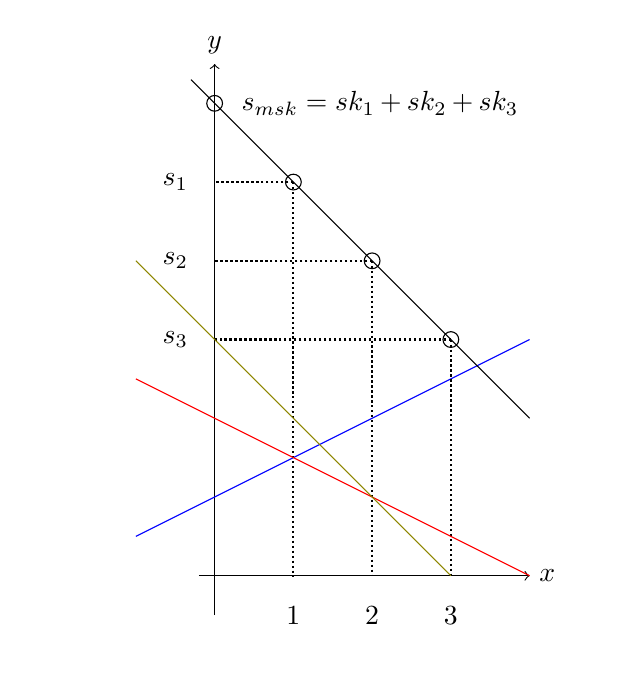
\begin{tikzpicture}[block/.style={rectangle,text width=10em,text centered,minimum height=9mm}]
\def\hZero{1}
\def\hOne{0.5}
\def\hTwo{0}
\def\hThree{2.5}
  \draw[->] (-0.2,0) -- (4,0) node[right] {$x$};
  \draw[->] (0,-0.5) -- (0,6.5) node[above] {$y$};
  %\draw[help lines] (-6,-5) grid (8,6);
\draw[scale=1,domain=-1:4,smooth,variable=\x,blue] plot ({\x},{1/2*\x+1});
\draw[scale=1,domain=-0.3:4,smooth,variable=\x] plot ({\x},{-\x+6});
%\draw (0,\hZero) circle (0.1cm);
\draw (3,3) circle (0.1cm);
\draw (2,4) circle (0.1cm);
\draw (1,5) circle (0.1cm);
\draw (0,6) circle (0.1cm);

\path
(-0.5,5) node [block] (spy1) {$s_1$}
(-0.5,4) node [block] (spy1) {$s_2$}
(-0.5,3) node [block] (spy1) {$s_3$}
(2.1,6) node [block] (spy1) {$s_{msk} = sk_1 + sk_2 + sk_3$}
(3,-0.5) node [block] (spy1) {3}
(2,-0.5) node [block] (spy1) {2}
(1,-0.5) node [block] (spy1) {1}
;

\begin{scope}[every path/.style=draw,densely dotted,thick]
\path (3,3) -- (0,3);
\path (3,3) -- (3,0);
\path (2,4) -- (0,4);
\path (2,4) -- (2,0);

\path (1,5) -- (0,5);
\path (1,5) -- (1,0);
\end{scope}
  %\draw[scale=0.5,domain=-3:3,smooth,variable=\y,red]  plot ({\y*\y},{\y});
  
  % Red graph
  \draw[scale=1,domain=-1:4,smooth,variable=\x,red] plot ({\x},{-1/2*\x+2});

\draw[scale=1,domain=-1:3,smooth,variable=\x,olive] plot ({\x},{-\x+3});
  
\end{tikzpicture}
}

\newpage

$sk_{msk} = sk_1 + sk_2 + sk_3$

\begin{equation}
e \left( Q_{privj, Alice}, P \right) = e \left( Q_{Alice}, P_{pubj} \right)
\end{equation}

\begin{equation}
P_{pub} = \sum_{ j= \{ 1,2 \} } b_j P_{pubj} \quad \textrm{for} \quad b_j = \prod_{z \in \{ 1,2 \} } \frac{z}{z-j}
\end{equation}

\begin{equation}
sk_{Alice} = \sum_{ j \in \{ 1,2 \} } b_j Q_{privj,Alice} \quad \textrm{for} \quad b_j = \prod_{z \in \{ 1,2 \} } \frac{z}{z-j}
\end{equation}

\begin{equation}
\rho = w_i \oplus H_2 \left( e \left( sk_{Alice}, U \right) \right)
\end{equation}

\begin{equation}
k = v \oplus H_3 \left( \rho \right)
\end{equation}

\begin{equation}
r = H_3 \left( \rho \parallel k \right)
\end{equation}

\begin{equation}
s_2 = \sigma_{2,3} + \sigma_{2,2} + \sigma_{2,1}
\end{equation}

\begin{equation}
s_1 = \sigma_{1,3} + \sigma_{1,2} + \sigma_{1,1}
\end{equation}



\end{document}
